\chapter{Performance Test}

As with many network protocols designed to transfer data quickly and reliably, there needs to be performance analysis. The performance of MCDTP is measured by throughput and packet loss.

\section{Test Environment}

The test environment was comprised of two servers rented from a cloud provider called DigitalOcean: a server in New York, USA and another server in Amsterdam, Netherlands. The rented servers were running Ubuntu 16.04 LTS and had the following configuration: 4 CPUs, 8GB of RAM, 80GB SSD, and 5 TB of transfer. The transfer specification is with respect to DigitalOcean tracking how much data passes through their network and imposing restrictions on rented servers. Unfortunately, DigitalOcean does not disclose any server specifications beyond this.

\section{Testing}

The executed tests used specific configurations. The implementation of MCDTPi was configured with single-, dual-, quad-, and octa-channel counts. Tests were also configured to load data from a 1GB data source. Even with this large data source, the available RAM allowed for the data to reside completely in memory. The role of client and server were arbitrarily assigned to the rented servers since both servers are perceivably identical. The Maximum Transmission Unit (MTU) for both servers were 1500 bytes. Fragmentation is not handled by MCDTP, so to avoid unpredictable behavior, MCDTPi was compiled to use a UDP packet size of 1400 bytes, to account for UDP packet headers.

\subsection{Test Results}

Throughput and packet loss were the metrics of focus while executing the tests. The built-in network logger was used to track packet loss and tcpdump was used to capture time and number of bytes as packets were transmitted and received. Both metrics were captured to file in real-time and later a custom built program was used to process the raw data. For instance, there were time gaps between transmitted packets that needed to be filled in as times where 0 bytes were sent. The raw data was also aggregated into one second intervals so that throughput could be calculated. For the following figures and tables, the aggregated data was further aggregated into 60 second intervals so that the behavior could be better observed.

The graphs in Figures \ref{fig:tr-ct} and \ref{fig:tr-st} show the throughput in Kilobits per second for single-, dual-, quad-, and octa-channel configurations for both client and server hosts, respectively. These results are discussed in Section \ref{sec:anlys}.

Tables \ref{tab:server-perf} and \ref{tab:client-perf} show further statistics on performance. Figures \ref{fig:tr-at}, \ref{fig:tr-mt}, and \ref{fig:tr-pl} are the graphical representation of this data. These results are discussed in Section \ref{sec:anlys}.

\begin{table}[H]
\centering
\caption{Server Performance}
\label{tab:server-perf}
\begin{tabular}{rcccc}
\multicolumn{1}{c}{} & Single    & Dual      & Quad       & Octa  \\
\hline
Average Throughput   & 17.9Kbps  & 18.1Kbps  & 2.7Kbps    & 0Kbps \\
\hline
Max Throughput       & 61.8Kbps  & 108.1Kbps & 146.3Kbps  & 0Kbps \\
\hline
Packet Loss          & 14.06\%   & 19.64\%   & 87.97\%    & 100\%
\end{tabular}
\end{table}

\begin{table}[H]
\centering
\caption{Client Performance}
\label{tab:client-perf}
\begin{tabular}{rcccc}
\multicolumn{1}{c}{} & Single    & Dual      & Quad       & Octa  \\
\hline
Average Throughput   & 15.9Kbps  & 14.9Kbps  & 2.6Kbps    & 0Kbps \\
\hline
Max Throughput       & 55.2Kbps  & 90.0Kbps  & 143.3Kbps  & 0Kbps
\end{tabular}
\end{table}


\section{Analysis}\label{sec:anlys}

The expected behavior of MCDTPi is that as resources increase with more channels, throughput and packet loss improve. The test results show that this behavior is partly true going from single-channel to dual-channel. Throughput improved two fold while packet loss had marginal degradation. However, performance worsened in both measurements for quad- and octa-channel configurations. Octa-channel was omitted in Figures \ref{fig:tr-ct} and \ref{fig:tr-st} because tests stalled and yielded no data. Though the Figure \ref{fig:tr-mt} shows quad-channel achieving the highest throughput, it had an average throughput that was half that of the single-channel. Quad-channel had over six times as much packet loss as well.

At the surface, this behavior seems to be inexplicable. When looking at the implementation of MCDTP, there is no bottleneck in the architecture that would cause packet transmission to be under-performant. Disk I/O operations occur asynchronously in such a way that does not interrupt the flow of data. If the issue does not exist within MCDTPi, then it must exist elsewhere.

As stated in Section \ref{sec:mod-arch}, the .NET Core Framework is the foundation for MCDTPi. It has a significant role in the performance of MCDTPi and warrants investigation. The TPL library was first to be inspected as it is key to asynchrony in MCDTPi and is a major component of the .NET Core Framework \cite{Leijen2009,netCore103Src}. The Common Language Runtime (CLR), the underlying runtime system that executes code written atop the .NET Framework and .NET Core Framework, reveals how TPL handles I/O operations \cite{richter2012clr}.

When the TPL library handles an I/O operation, it requests that the CLR use I/O Completion Ports (IOCP) to finish the I/O operation asynchronously \cite{richter2012clr}. The unique feature about IOCP is that it is a pool of threads (ThreadPool-IOCP) designated for waiting on I/O operations to complete so that the pool of threads (ThreadPool-TPL) used by TPL are used only for computation tasks. According to \cite{richter2012clr}, IOCP is part of the Win32 Kernel API (see \cite{netCore103Src} for more details).

The source code for the .NET Core Framework indicates that technology equivalent to IOCP for Unix based operating systems is not being used for non-Windows variants \cite{netCore103Src}. This means that I/O operations are handled by the TPL library and that computation tasks need to compete for resources against I/O operations. In scenarios where there are a significant number of asynchronous tasks, of both computation and I/O operations, the TPL library will under-perform. There is also the possibility that the TPL will deadlock if there are insufficient resources to handle the completion of an I/O operation as it must queue another task when the hardware signals the operation finished \cite{richter2012clr}.

This characteristic was not disclosed by \cite{netCore10,netCore103,netCore103Src} and thus this concern was not factored into the architecture of MCDTPi. Consequently, MCDTPi liberally used asynchrony to handle every packet that was transmitted and received. To transfer a 1GB data source requires more than 700,000 packets. The $Socket$ module uses four nested asynchronous computation tasks and an asynchronous I/O operation to handle a single packet. This means that transferring a 1GB requires 3.5 million asynchronous tasks for the $Socket$ module alone.

With so many task being scheduled on a system not fully optimized for asynchrony, the observed behavior of MCDTPi is now clear. The single-, dual-, and quad-channel configurations were able to operate since scheduled asynchronous tasks were more distributed. However, with each increase in channel count, the TPL library was put under strain more rapidly, negatively impacting performance. The octa-channel configuration overwhelmed the TPL library to the point of deadlock.


\newpage

\begin{figure}[ht]
\centering
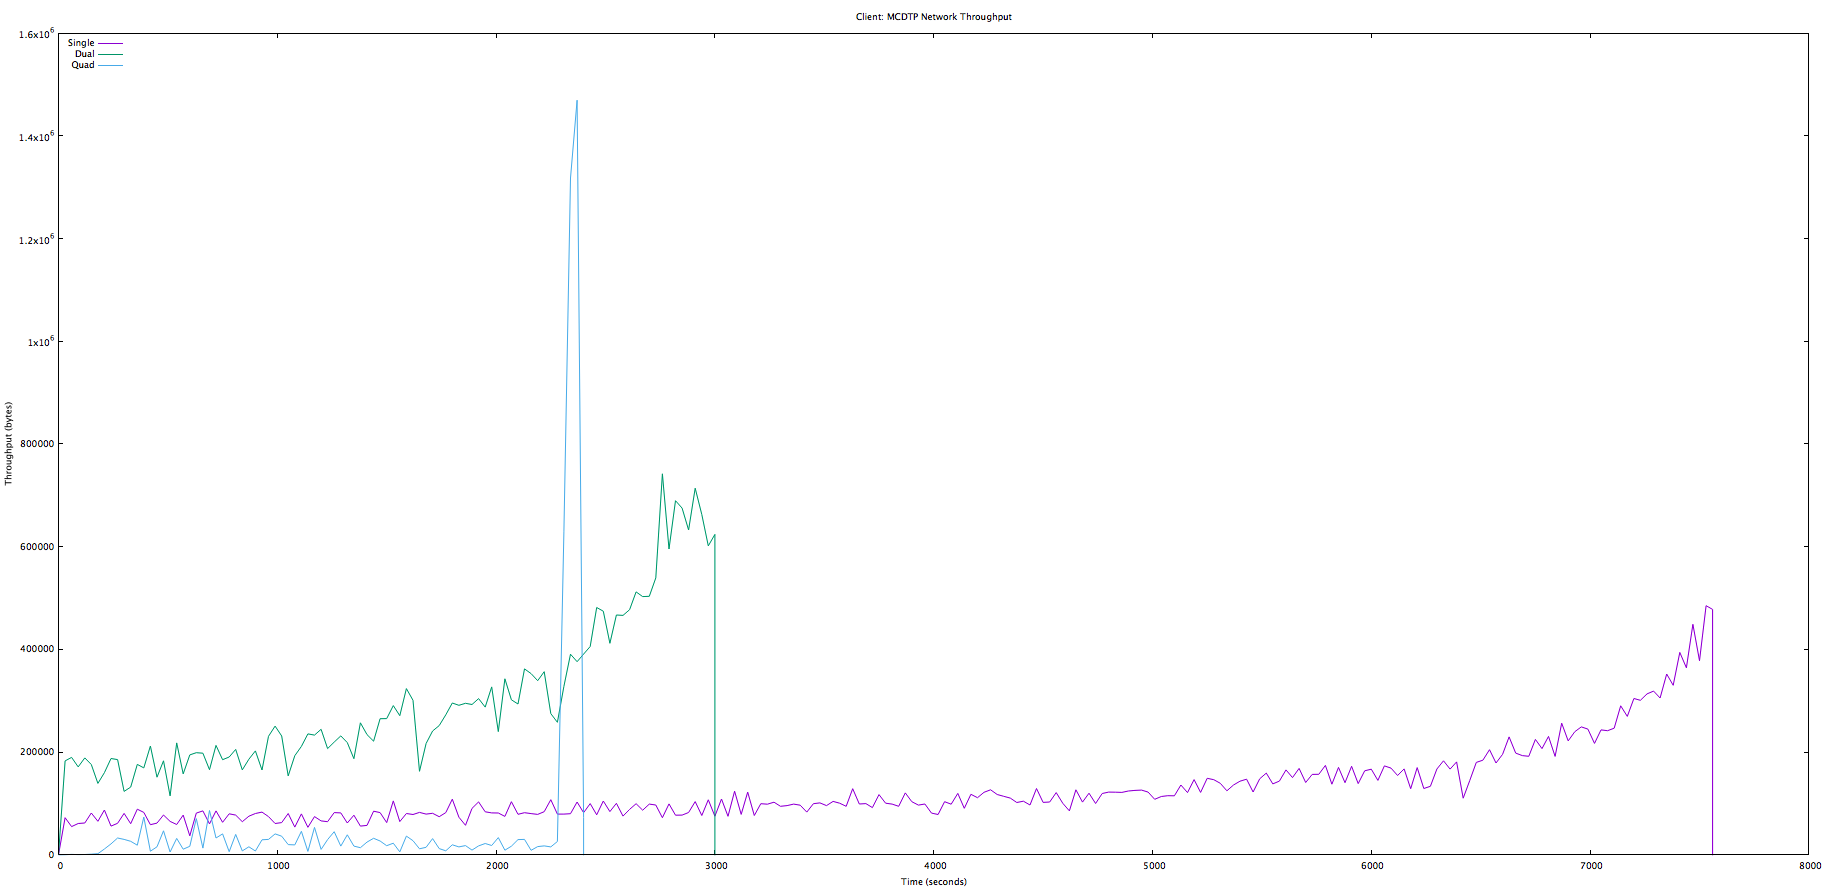
\includegraphics[scale=0.4]{TestResultClientThroughput}
\caption{Client Throughput}
\label{fig:tr-ct}
\end{figure}

\begin{figure}[ht]
\centering
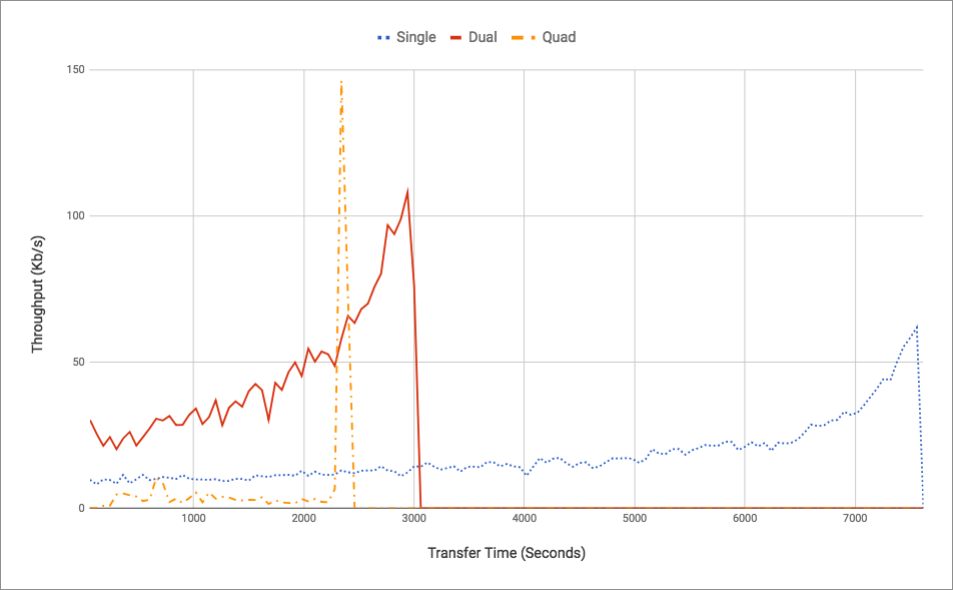
\includegraphics[scale=0.4]{TestResultServerThroughput}
\caption{Server Throughput}
\label{fig:tr-st}
\end{figure}

\begin{figure}[ht]
\centering
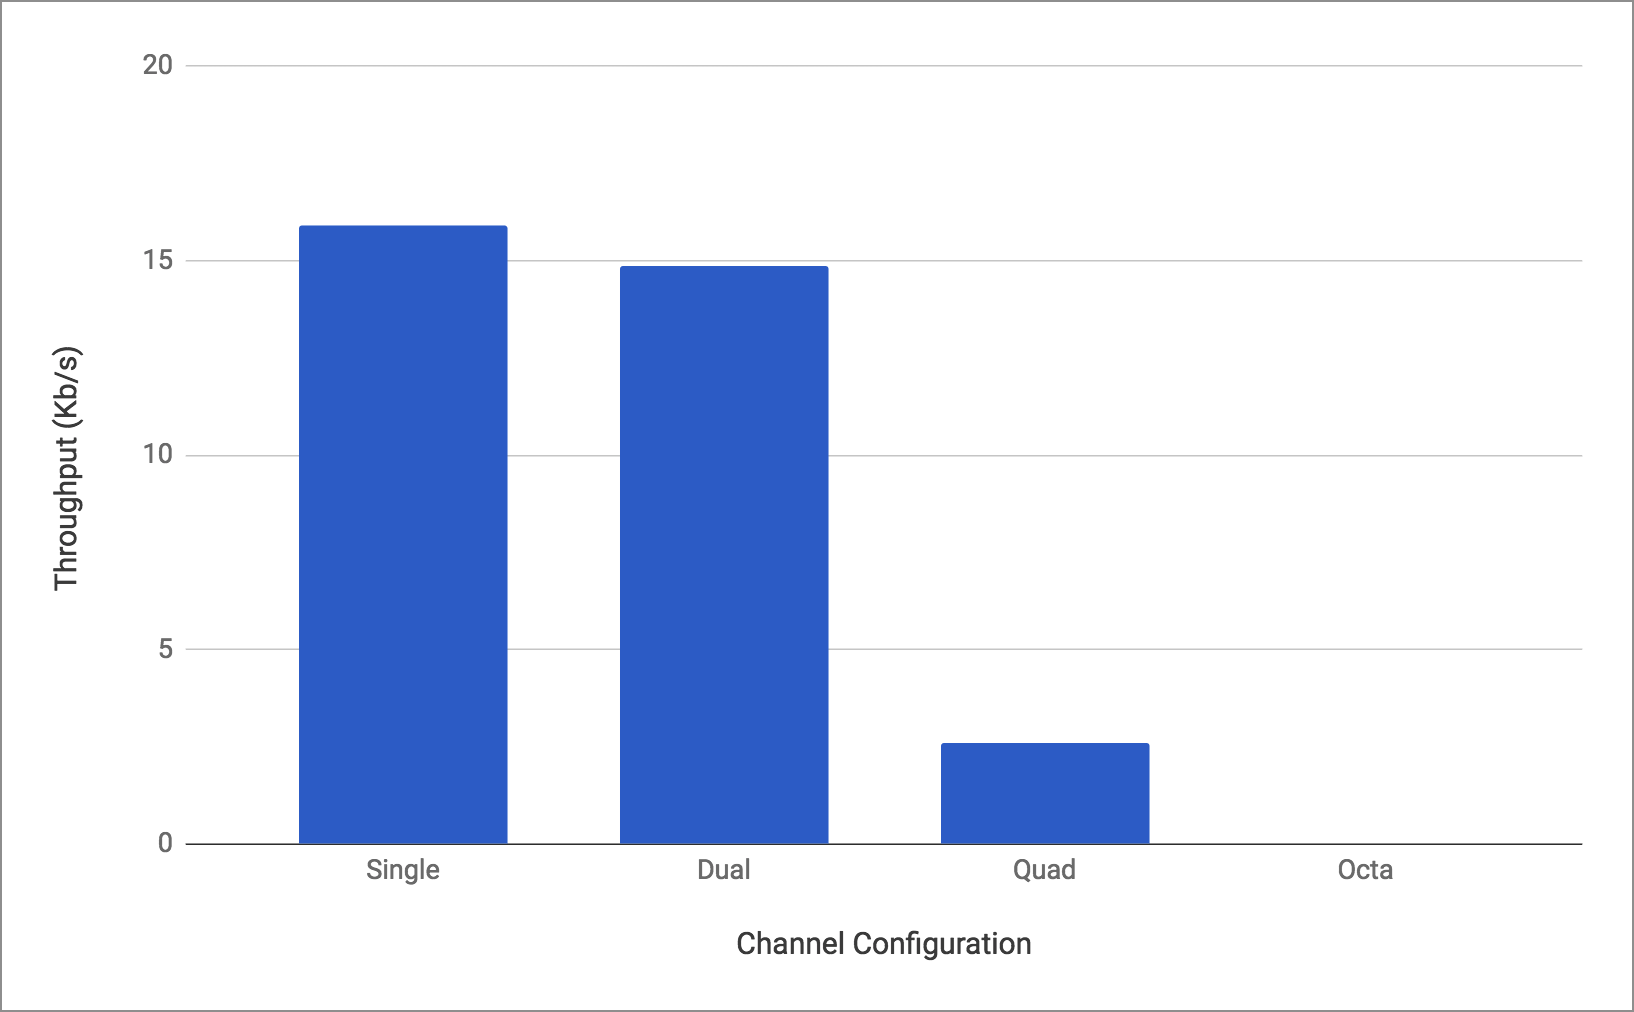
\includegraphics[scale=0.4]{TestResultAverageThroughput}
\caption{Average Throughput}
\label{fig:tr-at}
\end{figure}

\begin{figure}[ht]
\centering
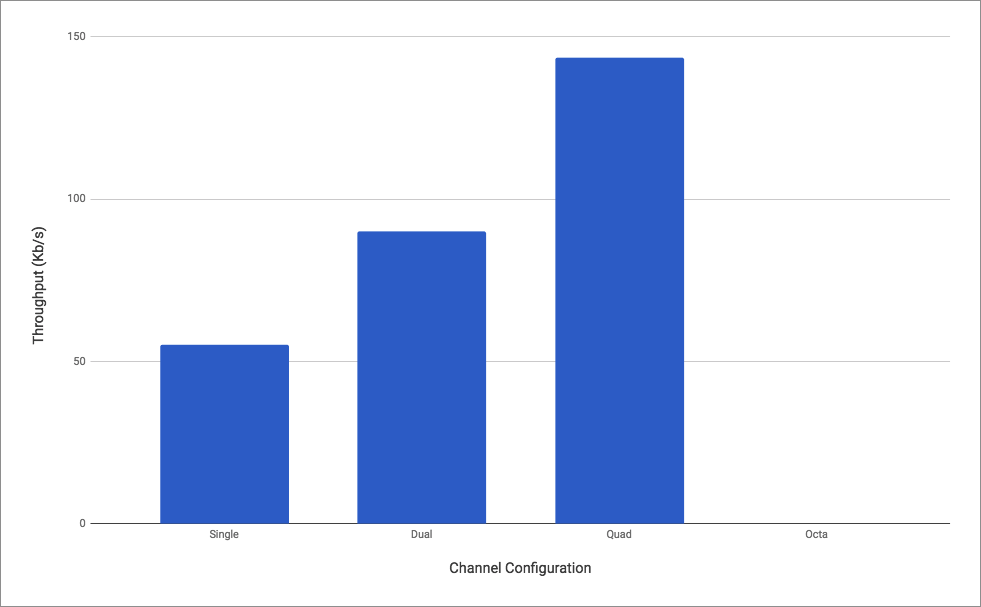
\includegraphics[scale=0.4]{TestResultMaxThroughput}
\caption{Max Throughput}
\label{fig:tr-mt}
\end{figure}

\begin{figure}[ht]
\centering
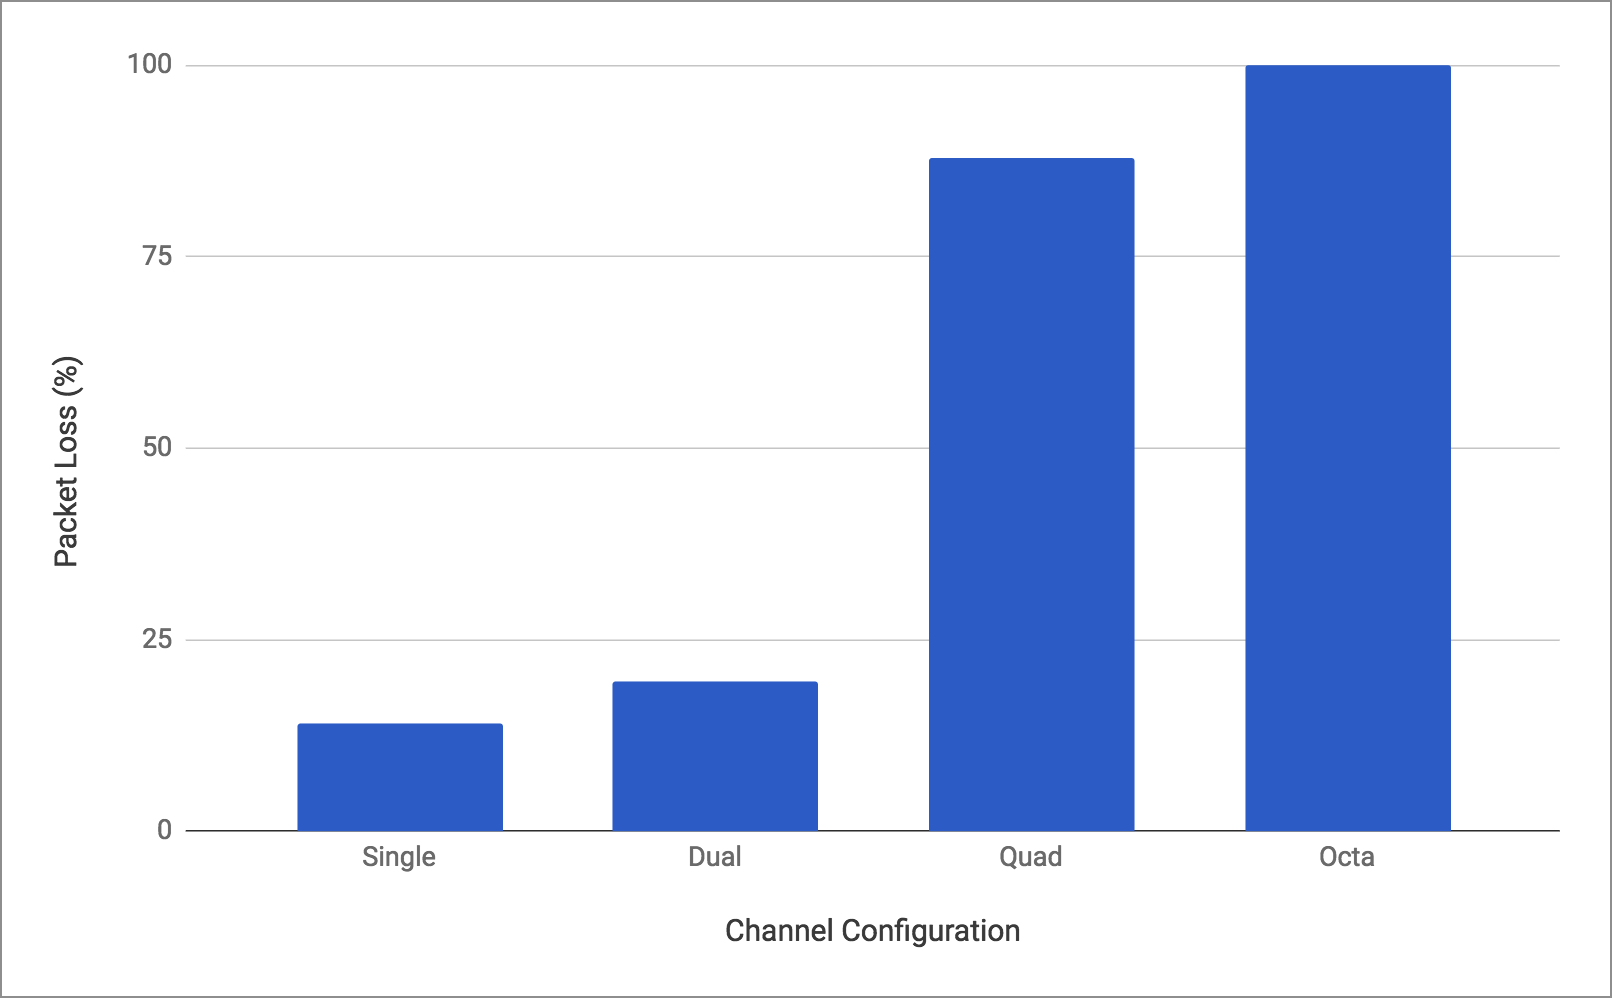
\includegraphics[scale=0.4]{TestResultPacketLoss}
\caption{Packet Loss}
\label{fig:tr-pl}
\end{figure}